\section{Modeling with differential equations} \label{S:7.5.Modeling}

\vspace*{-14 pt}
\framebox{\hspace*{3 pt}
\parbox{\boxwidth}{\begin{goals}
\item How can we use differential equations to describe 
  phenomena in the world around us?
\item How can we use differential equations to better understand these
  phenomena? 
\end{goals}} \hspace*{3 pt}}

\subsection*{Introduction}

In our work to date, we have seen several ways that
differential equations arise in the natural world, from the growth of
a population to the temperature of a cup of coffee.  In this section,
we will look more closely at how differential equations give us a
natural way to describe various phenoma.  As we'll see, the key is to
focus on understanding the different factors that cause a quantity to
change.

\begin{exercises} 
  \item  Congratulations, you just won the lottery!  In one option
    presented to you, you will be paid one million dollars a year for
    the next 25 years.  You can deposit this money in an account that
    will earn 5\% each year.

    \ba
  \item Set up a differential equation that describes the rate of
    change in the amount of money in the account.  Two factors cause
    the amount to grow---first, you are depositing one millon dollars
    per year and second, you are earning 5\% interest.

  \item If there is no amount of money in the account when you open
    it, how much money will you have in the account after 25 years?

  \item The second option presented to you is to take a lump sum of 10
    million dollars, which you will deposit into a similar account.  How
    much money will you have in that account after 25 years?

  \item Do you prefer the first or second option?  Explain your thinking. 

  \item At what time does the amount of money in the account under the
    first option overtake the amount of money in the account under the
    second option?
    \ea

  \item When a skydiver jumps from a plane, gravity causes 
    her downward velocity to increase at the rate of $g\approx 9.8$
    meters per second squared.  At the same time, wind resistance
    causes her velocity to decrease at a rate proportional to the
    velocity.  

    \ba
    \item Using $k$ to represent the constant of proportionality,
      write a differential equation that describes the rate of change
      of the skydiver's velocity.
    \item Find any equilibrium solutions and decide whether they are
        stable or unstable.  Your result should depend on $k$.
      \item Suppose that the initial velocity is zero.  Find the
        velocity $v(t)$.
      \item A typical terminal velocity for a skydiver falling face
        down is 54 meters per second.  What is the value of $k$ for
        this skydiver?
      \item How long does it take to reach 50\% of the terminal
        velocity? 
      \ea

    \item During the first few years of life, the rate at which a baby
      gains weight is proportional to the reciprocal of its weight.

      \ba
      \item Express this fact as a differential equation.

      \item Suppose that a baby weighs 8 pounds at birth and 9 pounds
        one month later.  How much will he weigh at one year?
      \item Do you think this is a realistic model for a long time?
        \ea

\item  Suppose that you have a water tank that holds 100 gallons of water.
  A briny solution, which contains 20 grams of salt per gallon, enters
  the tank at the rate of 3 gallons per minute.

  At the same time, the solution is well mixed, and water is pumped
  out of the tank at the rate of 3 gallons per minute.

\ba
\item Since 3 gallons enters the tank every minute and 3 gallons
  leaves every minute, what can you conclude about the volume of water
  in the tank.

\item How many grams of salt enters the tank every minute?

\item Suppose that $S(t)$ denotes the number of grams of salt in the
  tank in minute $t$.  How many grams are there in each gallon in
  minute $t$?

\item Since water leaves the tank at 3 gallons per minute, how many
  grams of salt leave the tank each minute? 

\item Write a differential equation that expresses the total rate of
  change of $S$.

\item Identify any equilibrium solutions and determine whether they
  are stable or unstable.

\item Suppose that there is initially no salt in the tank.  Find the
  amount of salt $S(t)$ in minute $t$.

\item What happens to $S(t)$ after a very long time?  Explain how you
  could have predicted this only knowing how much salt there is in
  each gallon of the
  briny solution that enters the tank.
\ea

\end{exercises}
\afterexercises




\subsection*{Developing a differential equation}

Preview activity~\ref{PA:7.5} demonstrates the kind of thinking we will be
doing in this section.  In each of the two examples we considered, there is a
quantity, such as the amount of money in the bank account or the
amount of salt in the tank, that is changing due to several factors.
The governing differential equation results from the total rate of change being the difference between the rate of
increase and the rate of decrease.

\bex \label{Ex:7.5.1}
In the Great Lakes region, rivers flowing into the lakes carry a great
deal of pollution in the form of small pieces of plastic averaging 1
millimeter in diameter.  In order to understand how the amount of
plastic in Lake Michigan is changing, construct a model for how this type pollution has built up in the lake.
\eex

First, some basic facts about Lake Michigan.
\begin{itemize}
  \item The volume of the lake is
    $5\cdot10^{12}$ cubic meters.
  \item Water flows into the lake at a rate of
    $5\cdot10^{10}$ cubic meters per year.  It flows out of the lake
    at the same rate.
  \item Each cubic meter flowing
    into the lake contains roughly $3\cdot10^{-8}$ cubic meters of
    plastic pollution.
\end{itemize}

Let's denote the amount of pollution in the lake by $P(t)$, where $P$
is measured in cubic meters of plastic and $t$ in years.  Our goal
is to describe the rate of change of this function;  in other
words, we want to develop a differential equation describing $P(t)$.

First, we will measure how $P(t)$ increases due to pollution flowing
into the lake.  We know that $5\cdot10^{10}$ cubic meters of water
enters the lake every year and each cubic meter of water contains
$3\cdot10^{-8}$ cubic meters of pollution.  Therefore, pollution
enters the lake at the rate of
$$
\left(5\cdot 10^{10} \frac{m^3 \mbox{\ water}}{\mbox{year}}\right) \cdot \left(3\cdot10^{-8} \frac{m^3 \mbox{\ plastic}}{m^3 \mbox{\ water}} \right) = 1.5\cdot 10^3\quad
\hbox{cubic m of plastic per year}.
$$

Second, we will measure how $P(t)$ decreases due to pollution flowing
out of the lake.  If the total amount of pollution is $P$ cubic
meters and the volume of Lake Michigan is $5\cdot 10^{12}$ cubic
meters, then the concentration of plastic pollution in Lake Michigan is
$$
\frac{P}{5\cdot10^{12}} \quad \hbox{cubic meters of plastic per cubic meter of water}.
$$
Since $5\cdot10^{10}$ cubic meters of water flow out each year\footnote{and we assume that each cubic meter of water that flows out carries with it the plastic pollution it contains}, then
the plastic pollution leaves the lake at the rate of
$$
\left(\frac{P}{5\cdot10^{12}} \frac{m^3 \mbox{\ plastic}}{m^3 \mbox{\ water}} \right) \cdot \left(5\cdot10^{10} \frac{m^3 \mbox{\ water}}{\mbox{year}} \right)=\frac{P}{100} 
\quad \hbox{cubic meters of plastic
  per year}.
$$

The total rate of change of $P$ is thus the difference between the rate at which
pollution enters the lake minus the rate at which pollution leaves the
lake;  that is,
\begin{eqnarray*}
\frac{dP}{dt} & = &1.5\cdot10^{3}-\frac{P}{100} \\
                   & = & \frac{1}{100}(1.5\cdot10^{5} - P).
\end{eqnarray*}

We have now found a differential equation that describes the rate
at which the amount of pollution is changing.  To better understand the
behavior of $P(t)$, we now apply some
of the techniques we have recently developed.

Since this is an autonomous differential equation, we can sketch
$dP/dt$ as a function of $P$ and then construct a slope field, as shown in Figure~\ref{F:7.5.Ex1}.

\begin{figure}[h]
\begin{center}
  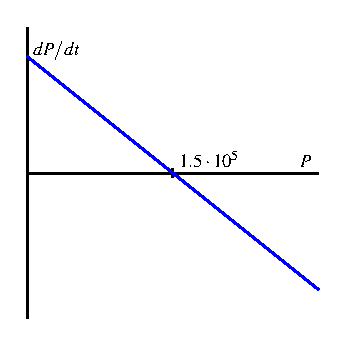
\includegraphics{figures/7_5_lake_michigan.eps}\qquad
  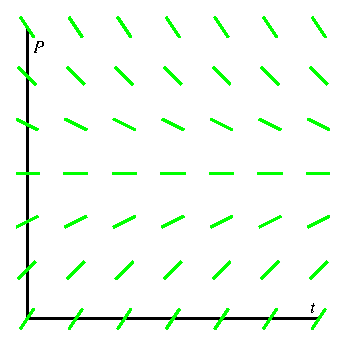
\includegraphics{figures/7_5_slope_field.eps}
\caption{Plots of $\frac{dP}{dt}$ vs. $P$ and the slope field for the differential equation $\frac{dP}{dt} = \frac{1}{100}(1.5\cdot10^{5} - P)$.} \label{F:7.5.Ex1}
\end{center}
\end{figure}

These plots both show that $P=1.5\cdot10^5$ is a stable equilibrium.  Therefore,
we should expect that the amount of pollution in Lake Michigan will
stabilize near $1.5\cdot10^5$ cubic meters of pollution.

Next, assuming that there is initially no pollution in the lake, we will
solve the initial value problem
$$
\frac{dP}{dt} = \frac{1}{100}(1.5\cdot10^{5} - P), \ P(0) = 0.
$$
Separating variables, we find that
$$
\frac1{1.5\cdot10^5-P} \frac{dP}{dt} = \frac1{100}.
$$
Integrating with respect to $t$, we have 
$$  \int \frac1{1.5\cdot10^5-P} \frac{dP}{dt}~dt = \int \frac1{100}~dt,$$
and thus changing variables on the left and antidifferentiating on both sides, we find that
\begin{eqnarray*}
  \int \frac{dP}{1.5\cdot10^5-P} &=& \int \frac1{100}~dt \\
  -\ln|1.5\cdot10^5 - P| & = & \frac1{100}t + C
\end{eqnarray*}
Finally, multiplying both sides by $-1$ and using the definition of the logarithm, we find that
\begin{equation} \label{E:7.5.Ex1C}  1.5\cdot10^5 - P = C e^{-t/100}.
\end{equation}
This is a good time to determine the constant $C$.  Since $P =
0$ when $t=0$, we have
$$
1.5\cdot 10^5 - 0 = Ce^0 = C.
$$
In other words, $C=1.5\cdot10^5$. 

Using this value of $C$ in Equation~(\ref{E:7.5.Ex1C}) and solving for $P$, we arrive at the solution
$$ P(t) = 1.5\cdot10^5(1-e^{-t/100}).$$
Superimposing the graph of $P$ on the slope field we saw in Figure~\ref{F:7.5.Ex1}, we see, as shown in Figure~\ref{F:7.5.Ex1a}
\begin{figure}[h]
\begin{center}
  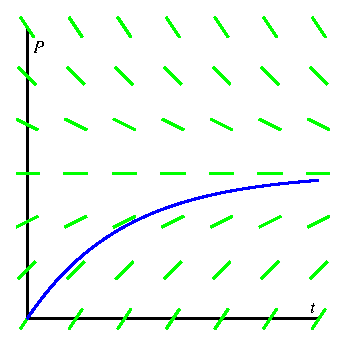
\includegraphics{figures/7_5_solution.eps}
\caption{The solution $P(t)$ and the slope field for the differential equation $\frac{dP}{dt} = \frac{1}{100}(1.5\cdot10^{5} - P)$.} \label{F:7.5.Ex1a}
\end{center}
\end{figure}
We see that, as expected, the amount of plastic pollution stabilizes around
$1.5\cdot10^5$ cubic meters.

\afterex

There are many important lessons to learn from Example~\ref{Ex:7.5.1}.  Foremost is how we can develop a differential equation by thinking about the ``total rate = rate in - rate out'' model.  In addition, we note how we can bring together all of our available understanding (plotting $\frac{dP}{dt}$ vs. $P$, creating a slope field, solving the differential equation) to see how the differential equation describes the behavior of a changing quantity.

Of course, we can also explore what happens when certain aspects of the problem change.  For instance, let's suppose we are at a time when the plastic pollution entering Lake Michigan has
stabilized at $1.5\cdot10^5$ cubic meters, and that new legislation is
passed to prevent this type of pollution entering the lake.  So, there is no longer any inflow of plastic pollution to the lake.  How does the amount of plastic pollution in Lake Michigan now change?  For example, how long does it take for the amount of plastic pollution in the lake to halve?

Restarting the problem at time $t=0$, we now have the modified initial value problem
$$
\frac{dP}{dt} = -\frac{1}{100}P, \ P(0) = 1.5\cdot10^5.
$$
It is a straightforward and familiar exercise to find that the solution to this equation is $P(t) = 1.5\cdot10^5
e^{-t/100}$.  The time that it takes for half of the pollution to flow
out of the lake is given by $T$ where $P(T) = 0.75\cdot10^5$.  Thus, we must solve the equation
$$0.75\cdot10^5 = 1.5\cdot10^5e^{-T/100},$$
or
$$ \frac12 = e^{-T/100}.$$
It follows that 
$$T = -100\thinspace\ln\left(\frac12\right) \approx 69.3 \quad\hbox{years.}$$

In the upcoming activities, we explore some other natural settings in which differential equation model changing quantities.

\newpage

\begin{activity} \label{A:7.4.finance}  
  Suppose you have a bank account that grows by 5\% every year.  Let $A(t)$ be the amount of money in the account in year $t$.

\ba
\item  What is the rate of change of $A$ with respect to $t$?

\item Suppose that you are also withdrawing \$10,000 per year.  Write
  a differential equation that expresses the total rate of change of
  $A$. 

\item Sketch a slope field for this differential equation, find any
  equilibrium solutions, and identify them as either stable or
  unstable.  Write a sentence or two that describes the significance
  of the stability of the equilibrium solution.

\item Suppose that you initially deposit \$100,000 into the account.  How
  long does it take for you to deplete the account?

\item What is the smallest amount of money you would need to have in
  the account to guarantee that you never deplete the money in the
  account? 
\item If your initial deposit is \$300,000, how much could you
  withdraw every year without depleting the account?

\ea
\end{activity}
\begin{smallhint}
\ba
	\item Small hints for each of the prompts above.
\ea
\end{smallhint}
\begin{bighint}
\ba
	\item Big hints for each of the prompts above.
\ea
\end{bighint}
\begin{activitySolution}
\ba
	\item Solutions for each of the prompts above.
\ea
\end{activitySolution}
\aftera

\begin{activity} \label{A:7.5.iv}  
A dose of morphine is 
        absorbed from the bloodstream of a patient at a rate
        proportional to the amount in the bloodstream.  

        \ba
        \item Write a differential equation for $M(t)$, the amount of
          morphine in the patient's bloodstream, using $k$ as the
          constant proportionality.
        \item 
          Assuming that the initial dose of morphine is $M_0$,
          solve the initial value problem to find $M(t)$.  Use the
          fact that the half-life for the absorption of morphine is
          two hours to find the constant $k$.
        \item Suppose that a patient is given morphine intraveneously
          at the rate of 3 milligrams per hour.  Write a differential
          equation that combines the intraveneous administration of
          morphine with the body's natural absorption.
        \item Find any equilibrium solutions and determine their
          stability. 
        \item Assuming that there is initially no morphine in the
          patient's bloodstream, solve the initial value problem to
          determine $M(t)$.  What happens to $M(t)$ after a very long time?
        \item To what rate should a doctor reduce the
          intraveneous rate so that there is eventually 7 milligrams
          of morphine in the patient's bloodstream?

\ea
\end{activity}
\begin{smallhint}
\ba
	\item Small hints for each of the prompts above.
\ea
\end{smallhint}
\begin{bighint}
\ba
	\item Big hints for each of the prompts above.
\ea
\end{bighint}
\begin{activitySolution}
\ba
	\item Solutions for each of the prompts above.
\ea
\end{activitySolution}
\aftera

\begin{summary}
\item Differential equations arise in a situation when we understand
  how various factors cause a quantity to change.
\item We may use the tools we have developed so far---slope
  fields, Euler's methods, and our method for solving separable
  equations---to understand a quantity described by a differential
  equation. 
\end{summary}

\nin \hrulefill

\begin{exercises} 
  \item  Congratulations, you just won the lottery!  In one option
    presented to you, you will be paid one million dollars a year for
    the next 25 years.  You can deposit this money in an account that
    will earn 5\% each year.

    \ba
  \item Set up a differential equation that describes the rate of
    change in the amount of money in the account.  Two factors cause
    the amount to grow---first, you are depositing one millon dollars
    per year and second, you are earning 5\% interest.

  \item If there is no amount of money in the account when you open
    it, how much money will you have in the account after 25 years?

  \item The second option presented to you is to take a lump sum of 10
    million dollars, which you will deposit into a similar account.  How
    much money will you have in that account after 25 years?

  \item Do you prefer the first or second option?  Explain your thinking. 

  \item At what time does the amount of money in the account under the
    first option overtake the amount of money in the account under the
    second option?
    \ea

  \item When a skydiver jumps from a plane, gravity causes 
    her downward velocity to increase at the rate of $g\approx 9.8$
    meters per second squared.  At the same time, wind resistance
    causes her velocity to decrease at a rate proportional to the
    velocity.  

    \ba
    \item Using $k$ to represent the constant of proportionality,
      write a differential equation that describes the rate of change
      of the skydiver's velocity.
    \item Find any equilibrium solutions and decide whether they are
        stable or unstable.  Your result should depend on $k$.
      \item Suppose that the initial velocity is zero.  Find the
        velocity $v(t)$.
      \item A typical terminal velocity for a skydiver falling face
        down is 54 meters per second.  What is the value of $k$ for
        this skydiver?
      \item How long does it take to reach 50\% of the terminal
        velocity? 
      \ea

    \item During the first few years of life, the rate at which a baby
      gains weight is proportional to the reciprocal of its weight.

      \ba
      \item Express this fact as a differential equation.

      \item Suppose that a baby weighs 8 pounds at birth and 9 pounds
        one month later.  How much will he weigh at one year?
      \item Do you think this is a realistic model for a long time?
        \ea

\item  Suppose that you have a water tank that holds 100 gallons of water.
  A briny solution, which contains 20 grams of salt per gallon, enters
  the tank at the rate of 3 gallons per minute.

  At the same time, the solution is well mixed, and water is pumped
  out of the tank at the rate of 3 gallons per minute.

\ba
\item Since 3 gallons enters the tank every minute and 3 gallons
  leaves every minute, what can you conclude about the volume of water
  in the tank.

\item How many grams of salt enters the tank every minute?

\item Suppose that $S(t)$ denotes the number of grams of salt in the
  tank in minute $t$.  How many grams are there in each gallon in
  minute $t$?

\item Since water leaves the tank at 3 gallons per minute, how many
  grams of salt leave the tank each minute? 

\item Write a differential equation that expresses the total rate of
  change of $S$.

\item Identify any equilibrium solutions and determine whether they
  are stable or unstable.

\item Suppose that there is initially no salt in the tank.  Find the
  amount of salt $S(t)$ in minute $t$.

\item What happens to $S(t)$ after a very long time?  Explain how you
  could have predicted this only knowing how much salt there is in
  each gallon of the
  briny solution that enters the tank.
\ea

\end{exercises}
\afterexercises


 




\clearpage
